\documentclass[journal]{IEEEtran}
\usepackage[T1]{fontenc}
\usepackage{etoolbox}
\patchcmd{\abstract}{---}{: }{}{}
\patchcmd{\IEEEkeywords}{---}{: }{}{}
\usepackage{amsmath,amssymb,graphicx,booktabs,array,tabularx,cite,url}
\usepackage[hidelinks]{hyperref}
\graphicspath{{images/}}
\setlength{\tabcolsep}{4pt}
\newcommand{\sys}{the combined controller}
\newcommand{\prov}[1]{\textit{Artifact source: #1.}}
\title{VIGILFOIL: Workload- and Response-Aware Evidence Accounting for Budgeted Security Monitoring in RPL Networks}
\author{Sharad Kumar Dubey, Vasim Khan\\
\small Department of Computer Science and Engineering\\
\small IIITDM Kancheepuram}
\begin{document}
\maketitle
\bstctlcite{IEEEcontrol}
\begin{abstract}
Legitimate computation and malicious activity can raise the same resource counters in an IoT device. Recovery actions create another source of ambiguity: redirecting a packet changes what the controller should expect on its original path. We address these two problems in VIGILFOIL, a gateway-based security controller for RPL networks. The gateway uses workload permissions to estimate normal resource demand. It records original and repaired delivery separately and checks whether an issued repair lease explains an omission. Host warnings then guide evidence requests and helper selection under a payload budget. We evaluated the accounting rules in native Cooja and tested the combined implementation in 42 runs with ten instruction-emulated Z1 motes. Response accounting reduced defense payload by 17.97\% in the native comparison. In the combined experiment, mean offered-work delivery reached 98.37\%, against 98.03\% for a network-only controller with the same instrumentation. The mean paired payload cost increased by 1.38\%. VIGILFOIL detected all four configured host-misuse episodes, but covered seven of ten sparse bursts. It also warned on 15.53\% of scored observations in complete benign runs. Thus, accounting can avoid unnecessary follow-up traffic, while benign host activity remains difficult to classify after integration.
\end{abstract}
\begin{IEEEkeywords}
Internet of Things, RPL, host-oriented mimicry, intrusion detection, evidence accounting, workload context, bounded recovery.
\end{IEEEkeywords}

\section{Introduction}
An IoT node may continue sending normal packets while it performs unauthorized work. Host-oriented mimicry attacks (HMAs) exploit this overlap between legitimate and malicious behavior. CIPHER~\cite{sanyal2026cipher} addresses HMA detection through collaboration between IDS nodes. Its placement and scheduling rules seek to keep collaborators available without running every IDS continuously. Our work starts from the same resource constraint, but examines the observations used to decide when further investigation is needed.

Two routine events illustrate the problem. A node receives a legitimate computation job, so its CPU activity increases. Later, the controller asks it to deliver some packets through a helper. The collector now receives fewer original packets. Both changes have an authorized cause. If the detector ignores the job, it may flag the CPU increase. If the controller ignores the redirect, it may query the node again to explain traffic that it deliberately moved.

Recovery can also conceal a failure. Receiving every item through a helper says little about whether the original path still works. We therefore retain the cause and route of each observation when enough supporting evidence is available. The question is whether this accounting changes the controller's communication cost and service outcomes under limited observation and repair budgets.

VIGILFOIL runs inference and policy decisions at a gateway. The motes measure their resources, report application work, and execute forwarding instructions. A warning raises the priority of a query and prevents the warned node from serving as a helper. It does not disconnect that node. This arrangement lets us test the effect of host evidence on the network response without claiming that the gateway stops a malicious process.

Our contribution has three parts. We define checks that distinguish submitted work, original receipts, and recovery through an authorized helper. We use independent workload permissions to interpret host-resource changes before requesting more evidence. We then measure the effects of these rules in closed-loop simulations, with component removals and simple controls. The new element we investigate is the connection between these records and the decisions they permit. The recurrent model, authentication, and repair mechanisms use established techniques.

\section{Related Work and Positioning}
\subsection{CIPHER and collaborative host monitoring}
CIPHER~\cite{sanyal2026cipher} addresses collaborator availability through IDS placement and scheduling, using host/network detection and a lightweight behavior monitor. CONTRAST~\cite{contrast} studies adaptive scheduling for host-based mimicry detection. LITMUS~\cite{sanyal2026litmus} extends collaborative HMA detection to settings with dishonest collaborators. These works establish that host evidence, temporal models, collaboration, and trust must be treated together. They are the closest lineage to our problem.

We adopt their motivation for using both host and network observations. We wrote the ledger, gateway transport, and repair controller used here. For the comparisons, we reconstructed the published detector components and the framework rules that were sufficiently specified. The authors' complete executable systems were not available to us. Table~\ref{tab:fidelity} states what each reconstruction preserves and where it differs.

Scheduling determines whether to execute an IDS. Our accounting rules determine what an observation can explain after the controller has acted. An authorized redirect can lower the expected original count, but a repaired receipt cannot establish original-path health. We test this distinction rather than claiming that context-aware detection or collaboration itself is new.

\subsection{Routing response and resource-constrained decisions}
SRF-IDS~\cite{srf} uses trust in routing decisions, and its source release~\cite{srfcode} allowed us to build a response baseline. Resource-bounded IDS scheduling has also been studied by Abbas et al.~\cite{abbas2015scheduling}. Observation control in quickest-change detection explicitly balances sampling and delay~\cite{decusum}. GRU-D uses missingness and time intervals in recurrent prediction~\cite{grud}. These works are relevant to our budget and temporal state, although VIGILFOIL's fixed priority rule has no corresponding optimality result.

A response may harm the traffic it is meant to protect. We tested this in native Cooja by placing the suspect relay on a bridge used by legitimate sources (Section~\ref{sec:support}). Offered delivery was 91.88\% with monitoring, 58.41\% with guarded exclusion, and 84.47\% when confirmation preceded exclusion. These are results from our controller experiment. They motivated the use of bounded repair instead of disconnection on a host warning alone.

\subsection{Temporal models and broader comparisons}
Sun, Johnsson, and Banerjee~\cite{radio} add TX/RX features to RPL statistics for LSTM detection. Lunderbye et al.~\cite{foundation} use a foundation model to classify RPL attacks. We used their released data and the official MOMENT implementation~\cite{momentcode} in a separate routing benchmark. This gives a recent temporal-model comparison, but the routing labels do not describe hidden host work.

The comparison has several parts because no single dataset provides all the required observations. We use HMA reconstructions for the closest detector comparison, a source port for SRF response, and public CSVs for routing classification. Live detector substitutions share our controller and observation schema. Their delivery outcomes can be compared within that setup; they do not rank the original published systems as a whole.

\begin{table*}[t]
\caption{Baseline provenance and the scope of our comparisons. All results reported in this paper are our measurements unless explicitly attributed to a source.}
\label{tab:fidelity}\centering\small
\begin{tabularx}{\textwidth}{>{\raggedright\arraybackslash}p{2.1cm}>{\raggedright\arraybackslash}p{4.7cm}>{\raggedright\arraybackslash}X}
\toprule Method & Implemented or reused elements & Boundary of the comparison \\
\midrule
CIPHER~\cite{sanyal2026cipher} & Correlation-grouped LSTM/FC autoencoder, monitor, and reconstructed scheduling/placement replay & Author implementation unavailable. Widths and some training/aggregation choices are reconstructed. Latest live panel substitutes a detector into our controller. \\
CONTRAST~\cite{contrast} & CPU/TX autoencoder and scheduling/aging reconstruction & Width and attack-threshold sensitivities are explicit choices. Sampling and deployment differ from the paper. \\
LITMUS~\cite{sanyal2026litmus} & Host AE, network ensemble, Bloom consistency, trust replay & Some training and forgetting details are unavailable. Native substitution uses network features, not the original full framework. \\
SRF-IDS~\cite{srf,srfcode} & Archived detector, trust, messages, and routing objective & Native Cooja/UDGM port replaces Whitefield/NS3. ABI, addressing, capacities, and receive-path behavior required declared adaptations. \\
Radio LSTM~\cite{radio,radiocode} & Pinned author class; hidden width 10; source-trained controls & Released data contain 14 RPL fields, not the full 18-feature radio view. Our measured-radio panel is a separate reconstruction. \\
MOMENT RPL~\cite{foundation,momentcode} & Official frozen pretrained encoder and trained linear head & Public-data experiment uses 14 channels; paper parameter counts imply nine. No claim of MCU execution or full-model live HMA response. \\
\bottomrule
\end{tabularx}
\end{table*}

\section{Network, Threat Model, and Evidence}
\subsection{Network and execution boundary}
We consider a low-power IPv6 network using RPL~\cite{rpl}. A radio root collects application packets and reports from sources and relays. A gateway has more compute and storage than a mote and maintains the evidence ledger. The final integrated experiment uses ten Z1 motes, including the root, under instruction emulation in Cooja~\cite{cooja}. Its unit-disk radio model has a 30 m transmission range and a 45 m interference range. Transmit success is configured as one; reception success is 0.90 for the benign context, one for mixed attacks, and 0.85 for sparse/loss attacks. Every mote runs the application and protocol firmware. The gateway runs on the host computer.

Packet loss and small mote memory limit the evidence available to the gateway. Queries and recovery packets also consume network capacity. We count that traffic explicitly. Mandatory reports remain separate from the query/repair reservation, so meeting the reservation does not imply a bound on total traffic. Payload bytes provide no direct measurement of radio energy.

\subsection{Adversary and trusted components}
The evaluated adversary executes unauthorized arithmetic work and may selectively drop transit packets. Sparse misuse uses brief recurring CPU bursts. Earlier experiments also cover control forgery, report loss, dishonest forwarding claims, and stronger helper dropping. Attack configuration is known to the evaluator; oracle events are not inputs to the gateway.

We trust the root, gateway, workload issuer, and resource monitor. The attacker may misuse the application or drop packets, but cannot replace a trusted monitor's counters in the main experiment. A valid tag establishes who sent a report; it does not establish whether the reported measurement is true. We assume benign startup when forming the initial resource reference. We do not test compromised roots, poisoned startup, or hardware attestation. The keys used in the simulations are laboratory fixtures.

We checked the ambiguity of intent in the three-Z1 task experiment (Section~\ref{sec:support}). We ran equal amounts of unannounced benign work and hidden malicious work. Each seed produced 55 identical result observations for the matched pair. Given that view, the gateway cannot distinguish the two intentions. We use ``unexplained'' to mean unsupported by its permissions and observations, not proven malicious. Stale or missing evidence remains unknown.

\subsection{Work and receipt semantics}
For source $i$ and a recently closed epoch $e$, the ledger retains offered work $O$, submitted work $U$, blocked work $B$, original attempts $P$, repair attempts $R$, redirected work $D$, and lease identity $\ell$. The source report must satisfy
\begin{equation}
O_{i,e}=U_{i,e}+B_{i,e}.
\end{equation}
Each report is checked for count consistency, freshness, sequence, nonce, and action scope. Work identifiers allow us to match receipts without counting multiple copies as multiple completed items. We write the original receipt set as $\mathcal{Y}^{o}$ and the repaired set as $\mathcal{Y}^{r}$. Their union measures completed service. Only $\mathcal{Y}^{o}$ provides direct evidence about the original path.

A lower original count is accepted only with supporting root-issued lease history. In compact notation, the expected original work is
\begin{equation}
E^{o}_{i,e}=\begin{cases}P_{i,e},&\text{validated redirection supports }P_{i,e},\\ U_{i,e},&\text{otherwise.}\end{cases}
\end{equation}
The unexplained original deficit is $d_{i,e}=\max(0,E^o_{i,e}-|\mathcal{Y}^{o}_{i,e}|)$. An unsupported claim of redirection cannot reduce this expectation. Missing evidence does not establish a zero deficit or a benign source.

Suppose a source submits ten items. A valid lease redirects four, leaving six original attempts. If six original receipts and four repair receipts arrive, all ten items have been delivered. Expecting ten original receipts would create four artificial deficits. Using only the union would hide whether recovery was needed. This example explains why the controller needs both records; it is not a measured run.

\section{Combined Decision Method}
\begin{figure*}[t]
\centering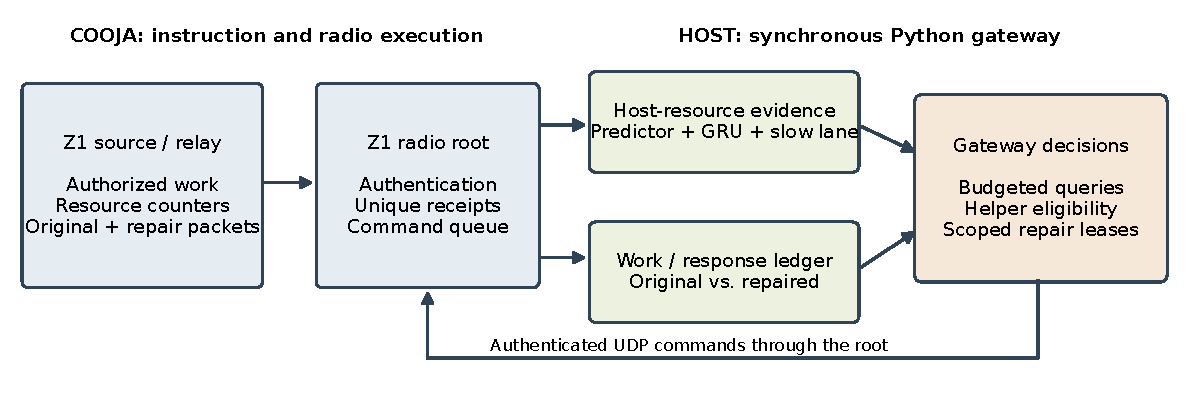
\includegraphics[width=.96\textwidth]{architecture.pdf}
\caption{Implemented evidence and action flow. Mote execution and packet transport occur in Cooja; inference and decision logic run in the Python gateway. Original and repaired receipts remain distinct. Ground-truth attack logs are used only by the evaluator.}
\label{fig:architecture}
\end{figure*}
\subsection{Workload-conditioned resource evidence}\label{sec:hostmethod}
Each mote reports cumulative CPU, TX, and RX ticks, RPL activity, own/transit counters, source time, and sequence. The root verifies the 84-byte host report and rejects wrong sessions or non-increasing sequences. The gateway forms causal differences only from received observations. Root-authorized work is separately bounded by amount and expiry; its permission is not inferred from the same resource anomaly it is meant to explain.

For measured CPU activity $c_t$, network context $x_t$, and authorized work $w_t$, the benign predictor is
\begin{align}
\widehat c_t &= f_{\mathrm{net}}(x_t)+\alpha w_t,\\
r_t &= c_t-\widehat c_t.
\end{align}
The network predictor and coefficient fit benign source deployments. CPU activity is the increment in active ticks divided by elapsed source time and 32,768; the final coefficient is $\alpha=3.219255\times10^{-5}$ in the implementation's activity-per-work units. TX and RX expectations are also predicted. Nine discriminator inputs describe observation timing/gaps, signed CPU/TX/RX residuals, and relative residuals. Source identities index state and attribution but are not numerical predictors.

A 16-unit GRU processes eight received observations. Its score is averaged with a histogram-gradient-boosting classifier score. At least three of the last five scores must exceed the neural threshold. We first trained this supervised head in the standalone Z1 host experiment described in Section~\ref{sec:support}, then retained its weights while refitting benign resource prediction and calibration for the combined network. We fitted the retained head in Python on ten Z1 source runs with 21,331 rows and 20,701 eight-observation windows; six development runs supplied 12,353 windows. The GRU used class-weighted binary cross-entropy, AdamW at 0.001, weight decay 0.01, batch 256, gradient clipping at one, and 100 epochs, retaining the checkpoint with minimum development loss. The histogram classifier used 150 iterations, 15 maximum leaf nodes, learning rate 0.05, and L2 regularization three. Thus its supervision differs from the benign-only autoencoders used as comparisons.

\subsection{Slow resource evidence}
A second lane retains moderate unexplained CPU activity across observations. Let $\sigma_t$ be a forwarding-rate-dependent noise scale with a relative expected-CPU floor, $b_i$ a bounded startup reference, and $\Delta t$ the received source-time gap. The implementation follows
\begin{align}
z_t &= \operatorname{clip}(r_t/\sigma_t-b_i,-3,5),\\
S_t &= \min\!\left(2h,\max\!\left(0,e^{-\widetilde{\Delta t}/120}S_{t-1}
 +(z_t-1)\frac{\widetilde{\Delta t}}{5}\right)\right),
\end{align}
where $\widetilde{\Delta t}=\min(15,\max(1,\Delta t))$ seconds and $h$ is the calibrated threshold. After eight-observation warm-up, the first 20 residuals establish the bounded reference. The startup reference is the median standardized residual clipped to $[-2,2]$. The recurrence is an engineering rule; no detection-delay optimality is claimed.

A warning from either lane persists for 30 seconds. We set both thresholds using complete benign calibration runs, placing them above the observed calibration maxima with fixed margins. The frozen thresholds are 0.103122 for the neural score and 21.118909 for slow evidence. The latter decays with a 120-second constant and cannot exceed twice its threshold. Calibration does not guarantee the same false-warning rate on a new deployment, and a poisoned startup can corrupt the reference.

\subsection{Evidence acquisition and repair}
Every ten seconds, the gateway orders sources using
\begin{equation}
\pi_i=10d_i+20a_i+\mathbf{1}(n_i\land m_i),
\end{equation}
where $a_i$ is a current host warning, $n_i$ is the network-priority alarm, and $m_i$ indicates missing current work evidence. This is a fixed policy rule, not a learned optimal scheduler. Host evidence can trigger investigation even when delivery appears normal. Repair requires a delivery deficit and source-work evidence.

We consider a helper only if the source advertises it as a neighbor. Its recent route must reach the root without a cycle or a return through the source. We reject candidates with a large observed forwarding deficit or a current host warning. This is an evidence-based eligibility check, not proof of helper honesty. Even a node holding a valid lease can refuse to forward.

The controller first inspects the epoch ending two decision intervals earlier and can use support from either of two preceding epochs. Without a source-work fact it uses a two-item default for investigation priority while retaining the unknown flag; it cannot authorize repair from that default. Work reports expire after 35 seconds and query replies after 20 seconds. A repair lease lasts ten seconds.

The gateway reserves at most 480 application bytes per decision. A query/reply reserves 136 bytes. A two-copy repair lease reserves 248 bytes: 120 control bytes, 72 source-copy bytes, and 56 helper-copy bytes. Root, source, and helper enforce authentication, nonce, scope, and quota checks. Mandatory periodic reports and workload permission traffic are charged outside this reservation. The limit bounds admitted discretionary work, not total security traffic.

\subsection{What the response accomplishes}
The gateway sends each selected instruction to the root queue. The root transmits it over UDP, and the receiving firmware performs the redirect or helper forward. We measure the resulting delivery. Host CPU misuse can continue after the warning because this implementation has no process-killing mechanism. Its responses investigate evidence and recover network delivery.

\section{Implementation and Experimental Protocol}
\subsection{Implementation details}
The final root and leaf firmware have 6,294 and 5,782 bytes of static RAM respectively. These values exclude worst-case stack and heap. Full source-work reports occupy 108 bytes; original application packets occupy 28 bytes; source repair packets occupy 36 bytes; helper forwards occupy 28 bytes. A four-entry root command queue is polled every 125 ms. Software AES is checked against a known vector, and the saved packet evidence is independently checked for authentication and command consistency.

The simulation bridge exchanges root records and command bytes synchronously with the gateway. Root polling and packet delays advance simulated time; gateway inference pauses it. Consequently, a host inference timing is not part of the simulated end-to-end latency. The study uses no FIT IoT-LAB hardware and makes no MCU inference or real-time qualification claim.

\subsection{Experimental tracks and units}\label{sec:tracks}
Table~\ref{tab:tracks} separates the experiments used below. We organize the experiments by the question tested and the execution environment, as summarized below. Native Cooja runs execute network/controller code without emulating MCU CPU instructions. Z1 runs emulate the firmware instructions. Python replays and public-data fits cannot substitute for either type of live response experiment.

\begin{table*}[t]
\caption{Experimental tracks and their execution environments. Counts are not interchangeable independent sample sizes.}
\label{tab:tracks}\centering\small
\begin{tabularx}{\textwidth}{>{\raggedright\arraybackslash}p{2.5cm}>{\raggedright\arraybackslash}p{3.2cm}>{\raggedright\arraybackslash}X}
\toprule Track & Environment and extent & Question and unit of evidence \\
\midrule
Controller accounting & Native Cooja; 887 accepted candidate runs, including five bring-up smokes & Main accounting contrast: 36 matched cases per variant, three deployment seeds. Scale, identity, nested-component, and stronger-helper panels remain separate. \\
Live model substitutions & Native Cooja with exported C inference; 126 runs & Seven detectors, 18 runs each, common 15 root-visible features and controller; CPU absent. \\
Original-feature observations & Instruction-emulated Z1; 58 observation runs, followed by Python fits/replay & Includes two-hour benign sources and ten-hour attack runs; replay scheduling is not on-mote neural execution. \\
Public routing benchmark & Released Cooja CSVs; Python training/inference & 960 selected runs from 1,200 public files; common five-class N20 subset uses matched 14-channel inputs and duplicate exclusions. \\
SRF source port & Native Cooja/UDGM; 72 one-hour runs & Blackhole subset, 5/10/15 detectors; original source with explicit platform and receive-path adaptations. \\
Combined system & Ten emulated Z1 motes plus Python gateway & Four source/calibration runs and 42 final 900-second runs; seven policies, three contexts, two deployment blocks. \\
\bottomrule
\end{tabularx}
\end{table*}

\subsection{Combined-system split and scenarios}\label{sec:combinedsetup}
Source deployments 1111 and 1112 supply benign resource and autoencoder fitting. Deployments 1113 and 1114 calibrate on benign loss and legitimate workload changes. They yield 2,276 source rows and 2,241 calibration rows. The earlier supervised GRU/classifier weights are retained, while preprocessing and thresholds for the new rig use source/calibration data only. Final seeds 1151 and 1152 are held out until freezing.

Each final run lasts 900 seconds. Application offers occur from 180 to 840 seconds, authorized work from 300 to 780 seconds, and configured attacks from 400 to 700 seconds. Seed 1151 uses the bypass layout with target 2; seed 1152 uses the grid layout with target 3. Each deployment has three contexts: benign authorized activity and disturbance; sustained 250-round hidden CPU work with selective forwarding; and 1,000-round CPU bursts lasting four seconds every 60 seconds, with legitimate traffic changes, selective forwarding, and nominal reception probability 0.85. One seed per topology confounds seed and topology, so the study measures two deployment blocks rather than general topology robustness.

Seven policies use the same transport and instrumentation: the combined controller; a network-only controller that ignores host warnings; CIPHER-style and CONTRAST-style autoencoders; and removals of workload context, action accounting, and slow evidence. The network-only control retains shadow host computation and telemetry to isolate policy influence. It does not represent the minimum-cost controller after removing host monitoring entirely.

The CIPHER-style adaptation uses correlation-grouped width-two LSTMs over 18 available fields, window 16, 250 epochs, batch 32, and Adam learning rate 0.05. The CONTRAST-style adaptation uses CPU/TX, width eight, window 32, 200 epochs, batch 256, and learning rate 0.001. Both train on benign new sources and calibrate three-of-five warnings on complete benign runs. These short fits and available schemas differ from the original distributed experiments. Component removals retain the full model's frozen weights and thresholds; they test dependence on components rather than separately optimized replacements.

\subsection{Supporting experiments and controls}\label{sec:support}
We used four smaller experiments to examine assumptions before combining the host and network controllers. All were conducted by us; they address specific design questions rather than supplying additional independent replications of the final comparison.

For witness sampling, we ran 900-second native Cooja simulations on a ten-node RPL chain. Sender 4 transmitted through suspect relay 3 to honest witness 2. The relay dropped 50\% of application packets during attack episodes. We varied legitimate bursts, reception loss, and an evader that recognized marked probes. Fixed 20-second probing and root-triggered probing with a mandatory 40-second audit used the same monitored segment. We scored 60-second histories with an eight-second acknowledgment deadline and benign-only calibration. A follow-up experiment replaced dedicated probes with ordinary application data and compared deterministic every-fourth-packet acknowledgments, keyed 25\% sampling, authenticated receipts, and root delivery counts. It used four test seeds and separate benign calibration seeds. These designs test observation availability and restricted evasion, not arbitrary witness compromise.

For response safety, we compared monitoring with temporary parent exclusion/restoration and confirmation before exclusion in native Cooja. We varied whether legitimate paths depended on the suspect relay. Offered work remained in the service denominator when exclusion made its destination unreachable. This design exposes collateral loss at bridge relays instead of treating reduced attacker traffic as a service gain.

For task integrity, we used ten-node, 900-second native Cooja runs. The gateway issued two eight-field jobs every ten seconds and knew the intended computation. Paired full-checking policies either left missing results unresolved or completed them locally, with a limit of 16 item computations per ten seconds. We evaluated correctness and completion within 30 seconds. Eight additional 900-second three-Z1 instruction-emulated runs checked the signed arithmetic protocol and matched benign/malicious workload ambiguity. This task contract is a separate extension, not a component of VIGILFOIL's final combined model.

For standalone host development, we collected CPU/TX/RX and workload observations from instruction-emulated Z1 runs, trained the head as described in Section~\ref{sec:hostmethod}, and evaluated fresh host-misuse episodes, legitimate activity, and intermittent bursts. We then transferred the retained head to the combined experiment in Section~\ref{sec:combinedsetup}, refitting its benign predictor and thresholds. Standalone and integrated results therefore measure different traffic and calibration conditions.

\subsection{Metrics and validation}
Offered-work delivery is
\begin{equation}
\mathrm{PDR}_{O}=\frac{|\mathcal{Y}^{o}\cup\mathcal{Y}^{r}|}{\sum_{i,e}O_{i,e}},
\end{equation}
with unique genuine identifiers and blocked/unreachable offers retained. Worst-source delivery is the minimum source fraction within a run, then averaged across runs. Defense cost sums attempted application payload for mandatory reports, authorization, queries/replies, grants, and repair copies. Retransmissions, PHY headers, and Joules are not inferred from that sum.

Host metrics distinguish episode hits, burst coverage, observation precision/recall/F1, pooled negative-observation false-positive rate (FPR), and warnings in entirely benign runs. Sparse coverage counts a warning during execution or within 15 source-seconds of the burst's last execution. A warning already active at onset can cover a burst without constituting a fresh detection. Onset delay uses the first actual hidden-work execution, recorded by independent oracle logging, rather than the configured nominal start alone.

Validation checks simulation completion, finite causal features, source-only fitting, offered/receipt joins, command authentication, reservation admission, and saved-model replay. The model hash was frozen before final runs; firmware hashes were checked per run. The gateway source hash was recorded after completion, although independent replay reproduced recorded actions. This weaker provenance point remains disclosed.

\section{Results}
\subsection{Response accounting reduces conditional protocol cost}\label{sec:accountresults}
Table~\ref{tab:native} reports the main native-controller panel: ten nodes, bypass/grid layouts, seeds 521--523, and six contexts covering activity, benign loss, gray dropping, burst dropping, probe-reactive dropping, and forgery. The action-unaware removal uses 30,424.6 bytes/run against 24,958.3 for the full controller. The reduction is 17.97\%, or 5,466.2 bytes/run. An exploratory bootstrap over three deployment-seed blocks gives 5,059.7--5,779.7 additional bytes for the unaware variant. With only three blocks, this interval should not be read as a general deployment guarantee. Delivery differs by only 0.057 percentage points, with uncertainty spanning benefit and harm.

\begin{table}[t]
\caption{Native Cooja controller ablations, 36 cases per row. Delivery is offered-work delivery; payload is bytes/run.}
\label{tab:native}\centering\small
\begin{tabular}{lrrr}\toprule
Variant & Delivery (\%) & Worst (\%) & Payload (B)\\\midrule
Full controller &97.525&93.350&24,958.3\\
Action accounting off&97.468&93.178&30,424.6\\
Without context&97.449&93.054&33,190.3\\
Model influence off&97.543&93.335&23,570.7\\
Without repair&97.342&92.601&24,815.7\\
Auth. checks off&96.486&84.007&27,067.6\\
Periodic (20 s)&97.819&93.636&32,076.0\\
Budget 136 B&97.347&92.595&22,645.8\\
Budget 960 B&97.584&93.329&29,293.0\\\bottomrule
\end{tabular}
\end{table}

Removing context also increases payload in Table~\ref{tab:native}. To examine ordering, we ran another 18-case comparison in which only priority ordering was disabled. Context, authentication, reporting, and redirect settings stayed fixed. The full controller used 41.61\% less payload. We also repeated action accounting in an earlier native implementation, using a main panel and a mesh holdout. Savings were 13.13\% and 28.46\%, while delivery changed by $+0.190$ and $-0.168$ percentage points. The cost effect recurs across these setups, but the delivery effect is not uniformly positive. We keep the cohorts separate.

Periodic reporting is a strong alternative. It reaches 97.819\% delivery and better mean worst-source delivery, at 7,117.7 more bytes/run. Disabling the learned priority model saves 1,387.7 bytes/run without a consistent service loss. We therefore cannot attribute the protocol benefit to learning alone. Evidence coverage is also incomplete: 88.53\% of ledger states in the full native controller remain unknown. Every audited strict explanation has a supporting causal direct receipt under our source-honesty assumptions. That check does not resolve the unknown states.

\subsection{Latest combined architecture}
\begin{table*}[t]
\caption{Closed-loop comparison and ablation in Cooja with ten instruction-emulated Z1 motes and the Python gateway. Each row contains the same six context/deployment cells. Host observations are correlated.}
\label{tab:combined}\centering\small
\begin{tabular}{lrrrrrr}\toprule
Policy & Delivery (\%) & Worst-source (\%) & Defense B/run & Episodes & Benign warnings/scored & Sparse coverage\\\midrule
Combined &98.37&94.19&133,901&4/4&322/2074&7/10\\
Network-only (instrumented)&98.03&91.92&132,095&--&--&--\\
CIPHER-style AE&98.01&92.43&132,137&0/4&58/1936&0/10\\
CONTRAST-style AE&97.93&92.35&132,261&0/4&40/1636&0/10\\
Without workload context&97.63&90.31&135,553&4/4&380/2090&10/10\\
Action accounting off&98.42&94.99&134,725&4/4&326/2083&7/10\\
Without slow evidence&98.24&92.94&132,802&1/4&195/2068&3/10\\\bottomrule
\end{tabular}
\end{table*}

In Table~\ref{tab:combined}, the combined system reaches 98.37\% mean delivery versus 98.03\% for the instrumented network-only controller. The paired mean difference is 0.336 percentage points, ranging from $-0.600$ to $+1.263$. Mean worst-source delivery rises from 91.92\% to 94.19\%. The mean paired defense-payload increase is 1.38\%. These are descriptive results across two blocks; some individual cells lose delivery.

The combined controller warns during all four configured host-misuse episodes. It covers seven of ten sparse bursts. Table~\ref{tab:exposure} reports first-execution delays and actual packet drops. The grid relay drops no packets in these runs because it carries no transit traffic to attack. We retain those runs as host-misuse tests. Forwarding exposure occurs in the bypass layout, with 12 drops in the mixed case and three in the sparse case.

\begin{table}[t]
\caption{Full combined model: actual attack exposure and onset delay (emulated Z1 plus gateway).}
\label{tab:exposure}\centering\small
\begin{tabular}{llrrr}\toprule
Layout & Context & Drops & Delay (s) & Bursts\\\midrule
Bypass & Mixed &12&41.09&--\\
Bypass & Sparse/loss &3&36.19&4/5\\
Grid & Mixed &0&18.17&--\\
Grid & Sparse/loss &0&129.14&3/5\\\bottomrule
\end{tabular}
\end{table}

\begin{figure*}[t]\centering
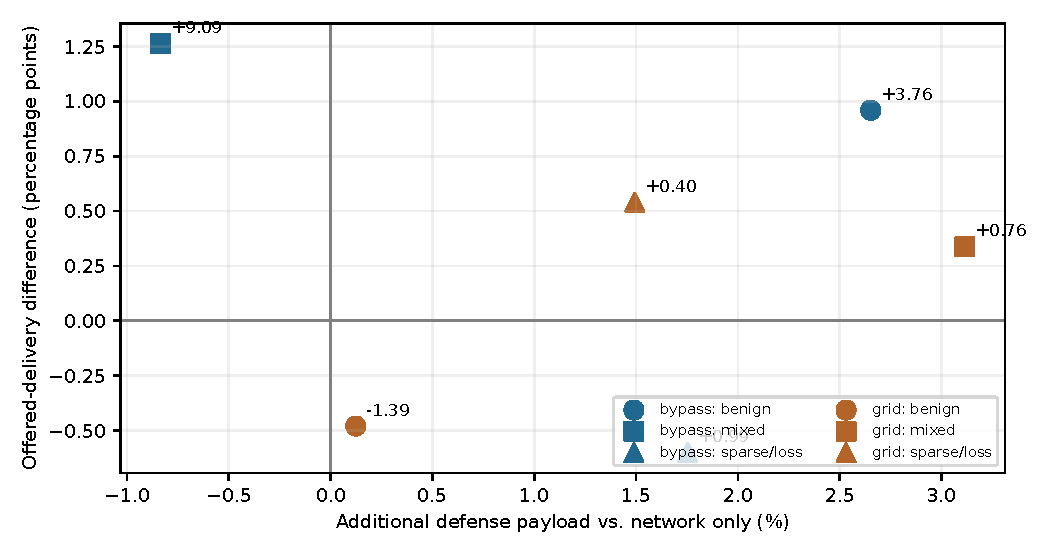
\includegraphics[width=.92\textwidth]{paired-tradeoffs.pdf}
\caption{Paired combined-versus-network-only outcomes for all six final Z1/gateway cells. Marker shape identifies context and color identifies deployment. Point annotations give the worst-source delivery difference in percentage points. Rightward movement costs more payload; upward movement improves offered delivery. The two deployment blocks are not independent topology replications.}\label{fig:paired}
\end{figure*}
Figure~\ref{fig:paired} retains each matched cell rather than hiding variation behind the mean. The worst-source annotations expose whether a change in average service also reaches the least-served source.

\subsection{Sensitivity is accompanied by false warnings}
At the frozen operating point, pooled host precision is 21.61\%, recall is 78.21\%, and F1 is 0.339 (Table~\ref{tab:detection}). The pooled negative-observation FPR is 11.03\%. In the two wholly benign runs, 322 of 2,074 scored observations trigger warnings, giving 15.53\%. These denominators differ: the pooled metric also includes labeled negative observations from attack runs and recovery. Neither rate measures independent alert incidents per hour.

\begin{table}[t]
\caption{Pooled host-observation metrics in the final Z1/gateway study. FPR uses all labeled negative observations.}
\label{tab:detection}\centering\small
\begin{tabular}{lrrrr}\toprule
Policy & Prec. (\%) & Rec. (\%) & F1 & FPR (\%)\\\midrule
Combined&21.61&78.21&.339&11.03\\
CIPHER-style&0.00&0.00&.000&1.85\\
CONTRAST-style&0.00&0.00&.000&1.80\\
Without work&22.77&100.00&.371&13.17\\
Without action&20.72&78.21&.328&11.62\\
Without slow evidence&8.52&12.88&.103&5.35\\\bottomrule
\end{tabular}
\end{table}

Without the slow accumulator, only one episode is hit and three sparse bursts are covered. Benign warnings fall to 195 from 322. This is a sensitivity-versus-warning trade-off. The GRU is still present in this removal, so the result concerns the added accumulator, not recurrent memory in general.

Providing workload permissions raises mean delivery and reduces warnings in complete benign runs from 18.18\% to 15.53\%. Yet the no-work variant has higher F1, 0.371, and covers all ten bursts. Inspection of its onset records explains why coverage alone is insufficient: all four attack runs already have a warning within 15 seconds before hidden work begins. Two sparse onset differences are negative. We count that as carryover, not anticipation of an attack.

Neither autoencoder substitution warns during the four host episodes at its frozen threshold. Both produce fewer benign warnings than the combined detector. Their training is benign-only, whereas our head uses attack labels and a separate residual accumulator. The common controller isolates their operational effect in this setup. It does not remove those differences in supervision or establish that the original CIPHER and CONTRAST frameworks are inferior.

\begin{figure*}[t]\centering
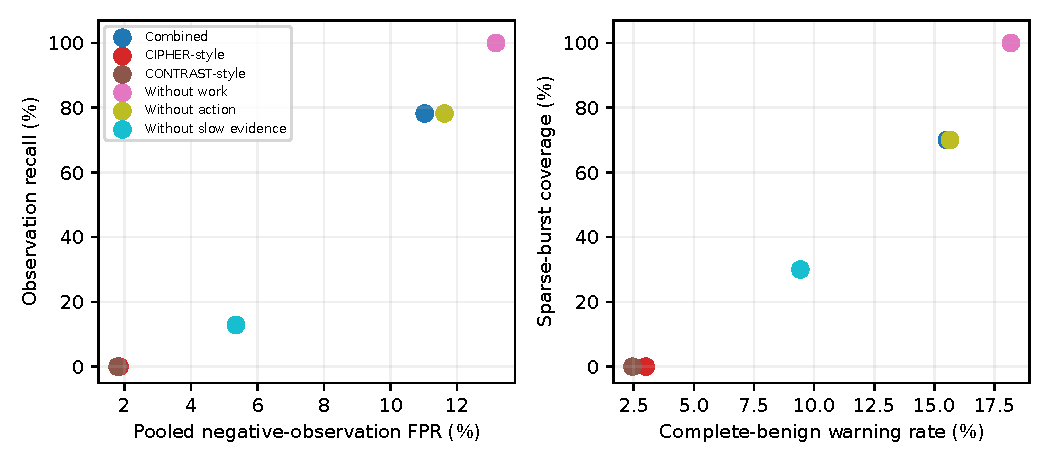
\includegraphics[width=.96\textwidth]{detection-tradeoffs.pdf}
\caption{Two operating-point views of the final Z1/gateway detector ablations. Left: pooled recall against pooled negative-observation FPR. Right: sparse-burst coverage against the complete-benign warning rate. These are frozen operating points, not ROC curves. Different denominators and pre-existing warning carryover prevent interpreting higher coverage alone as better discrimination.}\label{fig:dettrade}
\end{figure*}
Figure~\ref{fig:dettrade} makes the sensitivity cost visible: removing slow evidence reduces both warnings and coverage, while removing work context increases coverage together with benign warnings. These points do not establish an optimal operating frontier.

\subsection{Telemetry changes the cost balance}
The action-accounting effect is smaller after integration. Removing it increases mean paired payload by 0.61\% and slightly improves delivery to 98.42\%. The 17.97\% saving in Section~\ref{sec:accountresults} must therefore stay attached to the native experiment. Across the six full combined runs, host reports account for 600,264 of 803,404 defense bytes, or 74.715\%. Mandatory work reports add 128,304 bytes. Figure~\ref{fig:cost} shows that limiting repair and queries leaves most telemetry cost untouched.

\begin{figure}[t]\centering
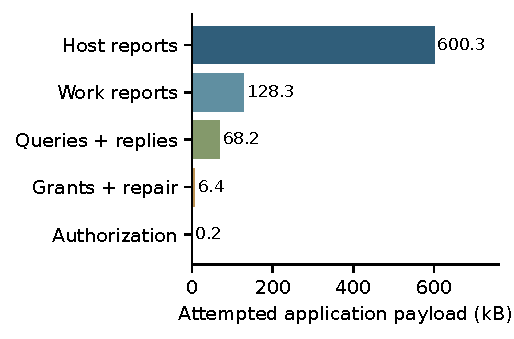
\includegraphics[width=\columnwidth]{cost-breakdown.pdf}
\caption{Attempted defense application payload across the six full-model Z1/gateway runs. Host and work reports dominate; the 480 B/decision cap applies only to discretionary reservations. Derived from recorded channels, not measured energy.}
\label{fig:cost}\end{figure}

The saved combined bundle is 1,432,961 bytes, including comparison models. Serialized components include a 1,173,474-byte predictor, a 227,415-byte classifier, and a 7,203-byte GRU state. The GRU has 1,313 parameters. A small recurrent cell is therefore not a small complete gateway artifact. In a same-input Python replay, 203 scored host reports have median processing time 5.13 ms and 95th percentile 5.53 ms. This is host wall time, not MCU latency. We do not compare these boundaries with a published detector-weight footprint as if they measured the same memory.

\begin{figure*}[t]\centering
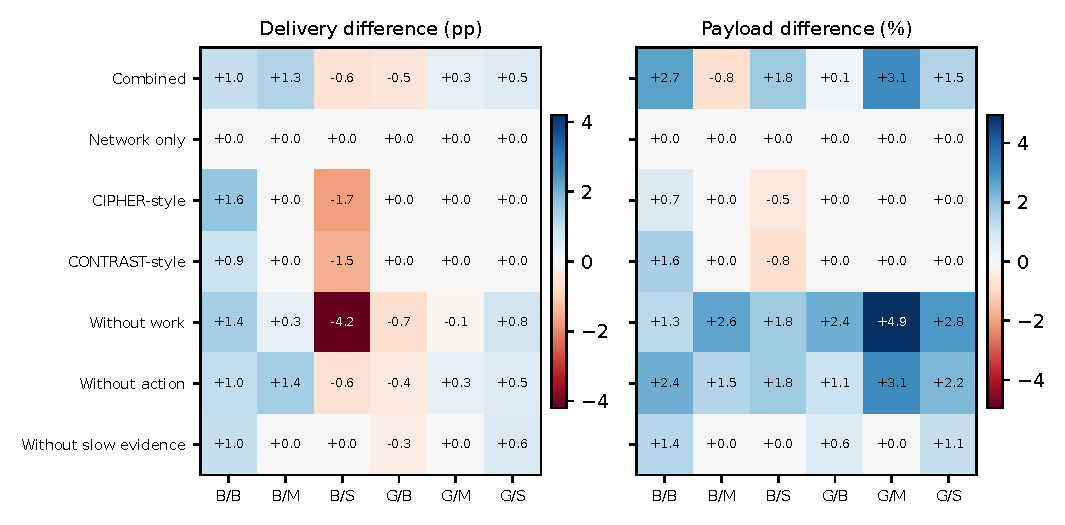
\includegraphics[width=.98\textwidth]{condition-matrix.pdf}
\caption{Condition-wise differences from the equally instrumented network-only control, using all 42 final Z1/gateway runs. B/B, B/M, B/S denote bypass benign, mixed, and sparse/loss; G denotes grid. Each cell compares the same deployment/context. Positive delivery differences improve service; positive payload differences increase cost. Color scales are panel-specific.}\label{fig:conditions}
\end{figure*}
Figure~\ref{fig:conditions} shows which ablation effects transfer across conditions. The aggregate differences in Table~\ref{tab:combined} should be read alongside these cells: neither the full model nor any removal dominates in every context.

\subsection{Broader live and public-data comparisons}
In the native live-substitution experiment summarized in Section~\ref{sec:tracks}, we tested seven detector choices under the same source-work, query, and repair controller. This panel uses seven detector choices on identical 15-feature root observations. CPU is absent, so the CONTRAST-style substitution uses TX/RX proxies. Table~\ref{tab:live} reports actual response outcomes, rather than counterfactual delivery inferred from offline scores. The LITMUS-style ensemble and frozen SGD controls are competitive; the CIPHER-style adaptation incurs more payload. Feature and supervision differences prevent transferring this ranking to the original frameworks.

\begin{table}[t]\caption{Separate native Cooja live detector substitutions, 18 runs per row. Common controller and 15 root features.}
\label{tab:live}\centering\small
\begin{tabular}{lrr}\toprule Detector & Delivery (\%) & Defense B/run\\\midrule
CIPHER-style AE&97.671&39,053.8\\
CONTRAST-style AE&97.830&27,862.0\\
LITMUS-style ensemble&97.887&27,941.3\\
Radio-LSTM architecture&97.872&26,088.0\\
Frozen SGD, fixed threshold&97.877&25,613.8\\
Frozen SGD, calibrated&97.844&25,876.4\\
Source-refitted SGD&97.741&30,448.7\\\bottomrule
\end{tabular}\end{table}

The public-data benchmark uses released RPL CSVs~\cite{radiocode}, Python training, 14 channels, 20-node runs, five classes, window 100, and stride 16. Five exact-content cross-split duplicate groups were found; three validation and two test files were excluded in the accepted rerun. Training copies remain disclosed. The effective MOMENT validation/test counts are 47/48. Splits group complete runs; overlapping windows are not randomly divided across training and testing.

\begin{table}[t]\caption{Separate public RPL classification benchmark (Python on released Cooja CSVs). These are routing-classification results, not the combined model's HMA results.}
\label{tab:public}\centering\small
\begin{tabular}{lrr}\toprule Model & Macro F1 & Fit-seed range\\\midrule
Official MOMENT-small + head&.8766&.8747--.8804\\
LSTM, hidden width 10&.5832&.5209--.6866\\
LSTM, current only&.4839&.4278--.5123\\
SGD with history&.7294&.7233--.7343\\
SGD, current only&.4667&.4328--.4882\\
Random forest, summaries&.7597&.7589--.7611\\
Dynamic INT8 LSTM&.4382&.4164--.4592\\\bottomrule
\end{tabular}\end{table}

MOMENT performs best on this benchmark, but the 14-channel adaptation has 35,373,253 parameters and 141,493,012 FP32 parameter bytes. The exact nine-channel smoke separately matches the source paper's parameter boundary. Its representation benefit does not imply mote feasibility. Temporal SGD and summary-based random forests also exceed the small LSTM. Dynamic INT8 reduces the tested LSTM's F1 from 0.5832 to 0.4382 and raises median host inference from 0.188 to 1.12 ms. Compression is therefore not an improvement in this measured configuration.

To test the value of added features, we collected a separate Z1 dataset using training seeds 561--563, validation seed 564, and test seeds 565--566. We transported CPU/TX/RX and work counters in 72-byte telemetry, formed causal 60-second statistics every five seconds, and compared nested 14/18/20/26-field inputs with source-only fitting. Python replay of those observations gives LSTM F1 values 0.5449 with 14 RPL fields, 0.4261 with radio features, 0.5086 with CPU added, and 0.5030 with work/freshness added. A supervised CPU-augmented SGD reaches 0.7062. These results show that more context is useful only when the model and transfer conditions make effective use of it. The collector is plain telemetry, not the final authenticated combined system.

\subsection{Original-feature replay and the SRF source port}
Long-duration Z1 observations help explain why framework reproduction and detector substitution cannot be combined into one score. Four ten-hour grid runs execute hidden work or staged false readings/file writes, but the compromised leaf has no incoming application-UDP rows in our collection. Two ten-hour chain runs provide feasible placement and about 43,000 incoming UDP rows at the observer. The workload case executes 28,799 work events, and the file case completes 2,459 CFS writes totaling 9,836 bytes. Framework decisions are then reconstructed in causal Python replay with 200-second cycles. Unavailable observations remain unknown. Collaboration counts are logical replay costs, not measured radio bytes.

The SRF comparison uses an independent native Cooja port, 30 benign clients, six malicious clients in attack runs, and 5/10/15 dedicated detectors in a $70\times70$ m deployment. Each detector setting has ten normal, ten SRF, and four malicious-MRHOF repetitions, each one hour long. Median all-client submitted PDR for SRF is 94.82\%, 98.32\%, and 96.48\%; the corresponding MRHOF values are 93.12\%, 92.39\%, and 90.58\%. All variants retain detector infrastructure. The metric includes malicious submissions and differs from our offered-work denominator. Recorded false-blacklist diagnostics in the SRF runs total 81, 93, and 125 respectively; these are repeated diagnostic events, not distinct falsely accused nodes. The result shows a response benefit in this declared port alongside collateral evidence, not a directly comparable score against the combined HMA controller.

\section{Lessons from the Wider Investigation}
The broader research included analytic, synthetic, native, and emulated experiments. Their value is in the design decisions they support, not in adding every run count to the final study.

First, we enumerated candidate node subsets on path and star graphs in Python to test whether the interpreted placement cardinality rule alone ensured coverage. This abstract-graph audit of the interpreted CIPHER cardinality rule found coverage holes in 15 of 70 examined path subsets and a star example with one internal node against a requested lower bound of five. These are Python graph counterexamples to that interpretation. They do not show that the authors' executable placement implementation fails. Placement was not retained as this paper's primary contribution.

Second, independent witnesses and adaptive sampling did not automatically outperform inexpensive counts. In our witness-sampling experiments (Section~\ref{sec:support}), fixed and triggered observation each achieved 11/16 detections within 60 seconds. The authenticated real-data sampling experiment gave 41/48 for both authenticated acknowledgments and source counts, while their negative-observation rates were 6.04\% and 0.50\%. These exploratory deadlines were measured relative to nominal attack phases, whereas the final combined study uses first actual execution. They are design-screening outcomes, not estimates of the final detector's accuracy.

Third, we screened adaptation and response alternatives using 24 native Cooja runs and a separate Python factorial model. The native runs tested source-trained detection under new grid/ladder conditions. In the model, we crossed bounded alternate delivery, two-observation confirmation, delayed benign-offset updates, and capped verification queues under paired traffic/noise, producing 7,680 factorial and sensitivity records. Alternate delivery and confirmation accuracy were model assumptions, not measured radio behavior. Sparse adaptation did not improve target detection, and some deferral combinations increased malicious exposure while improving modelled service. Synthetic assumptions cannot certify the live controller. We consequently retained explicit unknowns and bounded investigation, rather than presenting delayed decisions as a general open-set solution.

Fourth, in the task-integrity experiment defined in Section~\ref{sec:support}, we compared full checking with and without local completion of missing results. Fallback raised correct completions from 1,712/1,760 to 1,760/1,760 at 2.8\% extra item computations. For this toy workload, central execution is an easy and strong alternative. The task verifier is not part of the final combined architecture, and task correctness does not prove absence of hidden host activity.

Finally, in the standalone host experiment described in Section~\ref{sec:support}, we detected five of five fresh episodes with zero warnings among 8,239 scored benign observations, but covered only one of ten sparse bursts. The final integration changes the predictor, traffic, and conditions and produces substantial benign warnings. The older zero-warning result cannot be substituted for the current result. This transfer gap is one of the most useful findings of the development process.

\section{Limitations and Research Implications}
The main result is that records of authorized work and issued responses can change which deficits a controller investigates. We have implemented that connection and measured a communication benefit in the native study. The result is conditional on the traffic and trust assumptions. It is not an optimal acquisition policy, and the present comparison does not establish the absence of every overlapping method in prior work.

False warnings are the main obstacle to using the host detector. Precision of 21.61\% and a 15.53\% warning rate in benign runs do not support reliable HMA recognition. The integrated predictor must better handle forwarding load, workload-permission timing, and warning tails. A useful next comparison is a simple residual or linear model with the same workload information. That would test whether the GRU/classifier combination earns its extra complexity.

We tested the final model in two deployment blocks. Each topology has only one seed, so their effects are confounded. Repeated observations within a run do not increase the number of independent deployments. Some attack configurations also lack forwarding exposure. The broader model panels help identify transfer problems, but their different features and supervision prevent a single overall ranking.

Authentication cannot repair a dishonest measurement source. Our forged-counter test fails when a compromised source signs false measurements, and we provide no protected monitor. We also found a reset-state issue in a constructed Python fixture: the wrapper clears its state after a counter discontinuity, but the wrapped host detector retains its own state. The final runs did not include a reset campaign. A corrected version needs new validation before we can claim reboot or counter-reset robustness.

Several deployment costs remain unmeasured. Gateway computation pauses the simulation, static RAM excludes peak stack/heap use, and payload totals omit PHY overhead and retransmissions. We have no hardware energy, timing, or FIT IoT-LAB measurements. Reducing report frequency may lower the dominant telemetry cost, but it also makes evidence older and can hide short bursts. That trade-off needs a fresh experiment.

\section{Conclusion}
VIGILFOIL records authorized work and delivery recovery before deciding which anomalies need further evidence. Original receipts remain separate from repairs, and only a supported redirect can lower the expected original count. Our native Cooja comparison shows a 17.97\% defense-payload saving from this accounting. In the ten-Z1 combined experiment, mean delivery improves slightly, four host episodes are hit, and seven of ten sparse bursts are covered. Those gains come with substantial benign warnings and additional telemetry cost. The accounting result is useful, but the current host detector still needs better benign specificity and broader deployment testing.

\bibliographystyle{IEEEtran}
\bibliography{references}
\end{document}
